\documentclass[a4paper,14pt]{article}

%\usepackage{polyglossia}                          % Поддержка многоязычности
%\usepackage[T2A]{fontenc}                         % Поддержка русских букв
%
%\documentclass[14pt]{extarticle}
\usepackage{extsizes}
%\usepackage[linesnumbered,boxed]{algorithm2e}
\usepackage[linesnumbered,ruled,vlined]{algorithm2e}
\SetAlgorithmName{Алгоритм}{алгоритм}{Список алгоритмов}
\usepackage[top=2cm, bottom=2cm, left=3cm, right=1.5cm]{geometry}
%\renewcommand{\baselinestretch}{1.5}
\linespread{1.3}
\usepackage[utf8]{inputenc}                       % Кодировка utf8
\usepackage[english,russian]{babel}  
\usepackage{graphicx}
\usepackage{hyperref}
\usepackage{paralist} 
\let\itemize\compactitem
  \let\enditemize\endcompactitem
  \let\enumerate\compactenum
  \let\endenumerate\endcompactenum
  \let\description\compactdesc
  \let\enddescription\endcompactdesc
  \pltopsep=\medskipamount
  \plitemsep=1pt
  \plparsep=1pt % or \setlist{noitemsep} to leave space around whole list
\frenchspacing
\usepackage{fontspec}
\setmainfont[
BoldFont=timesbd.ttf,
ItalicFont=timesi.ttf,
BoldItalicFont=timesbi.ttf
]{times.ttf}  % Times New Roman
\usepackage{indentfirst}
\setlength{\parindent}{1.25cm}
\begin{document}

\begin{titlepage}
        \begin{center}
        ПРАВИТЕЛЬСТВО РОССИЙСКОЙ ФЕДЕРАЦИИ\\
        ФЕДЕРАЛЬНОЕ ГОСУДАРСТВЕННОЕ АВТОНОМНОЕ ОБРАЗОВАТЕЛЬНОЕ УЧРЕЖДЕНИЕ\\
        ВЫСШЕГО ПРОФЕССИОНАЛЬНОГО ОБРАЗОВАНИЯ\\
       «НАЦИОНАЛЬНЫЙ ИССЛЕДОВАТЕЛЬСКИЙ УНИВЕРСИТЕТ\\“ВЫСШАЯ~ШКОЛА~ЭКОНОМИКИ”»
        \\
        \bigskip
        Московский институт электроники и математики\\
        Департамент компьютерной инженерии\\
        Вдовкин Василий Алексеевич\\
        \bigskip
        \textbf{Разработка программы для поиска кратчайшего пути на карте с учетом препятствий}\\
        \bigskip
        Междисциплинарная курсовая работа по направлению подготовки 09.03.01~«Информатика и вычислительная техника»\\
        студент группы № \underline{ИВТ-11}\\
        (образовательная программа «Информатика и вычислительная техника»).\\
        \bigskip
        \bigskip
        \bigskip
        \end{center}
        \begin{flushright}
            Научный руководитель\\
            Ассистент Романов Александр Юрьевич\\
            \rule{11em}{.1pt}
        \end{flushright}
        \vfill\center{Москва 2015}
        
    \end{titlepage}
\tableofcontents %ОГЛАВЛЕНИЕ
\pagebreak
\section{Аннотация}


\subsection{Русский}

\subsubsection{Основная цель}
Исследование алгоритмов, позволяющих определить кратчайший путь между двумя вершинами в графе. Их практическое применение на примере карты с препятствиями. 

\subsubsection{Задачи}
Реализация программы на любом языке программирования, визуализирующей работу рассматриваемых алгоритмов поиска кратчайшего пути.

\subsubsection{Результаты}
Реализована программа на языке JavaScript, позволяющая:
\begin{itemize}
  \item Найти кратчайший путь между двумя точками на карте, если он существует.
  \item Оценить время работы алгоритма, количество обработанных вершин, существование оптимального пути и его длину.
  \item Изучить и сравнить алгоритм A* и алгоритм Дейкстры на основе визуализации их работы.
  \item Изменять размер карты и её топологию.
  \item Выбирать начальную и конечную точку, если они не являются препятствиями.
\end{itemize}

\subsubsection{Рекомендации}
\begin{itemize}
  \item Имеется начальная карта с размещёнными препятствиями, начальной точкой и конечной точкой пути.
  \item Начальная и конечная точки должны находятся внутри карты.
  \item Конечная точка должна быть пустой.
\end{itemize}



\subsection{English (WIP)}

\subsubsection{The main objective}
Исследование алгоритмов, позволяющих определить оптимальный путь между двумя вершинами в графе.

\subsubsection{Tasks}
Реализация программы на любом языке программирования, визуализирующей работу рассматриваемых алгоритмов поиска оптимального пути.

\subsubsection{Results}
Реализована программа на языке JavaScript, позволяющая:
\begin{itemize}
  \item Найти кратчайший путь между двумя точками на карте, если он существует.
  \item Оценить время работы алгоритма, количество обработанных вершин, существование оптимального пути и его длину.
  \item Изучить и сравнить алгоритм A* и алгоритм Дейкстры на основе визуализации их работы.
  \item Изменять размер карты и её топологию.
  \item Выбирать начальную и конечную точку, если они не являются препятствиями.
\end{itemize}

\subsubsection{Recomendations}
\begin{itemize}
  \item Имеется начальная карта с размещёнными препятствиями, начальной точкой и конечной точкой пути.
  \item Начальная и конечная точки должны находятся внутри карты.
  \item Конечная точка должна быть пустой.
\end{itemize}
\pagebreak
\section{Введение}
Поиск пути является одной из важнейших задач в теории графов. Решение данной задачи имеет широкое практическое применение в современных технологиях. В любой сфере разработки, в которой рабочее пространство можно представить в виде графа, реализация поиска пути является одним из основных аспектов.

Представление сети дорог ориентированным графом с положительными весами и возможностью изменения веса ребер позволяет разработчикам картографических сервисов решить данную задачу с учетом расположения физических объектов, длины дорог, их типа, проходимости, наличия пробок. Алгоритмы маршрутизации, с помощью которых информация находит свой путь от одного устройства к другому, также основываются на теории графов и задаче поиска пути. Создание искусственного интеллекта во многих играх не обходится без поиска пути между объектами на игровой карте.

Первые алгоритмы, позволяющие оптимально решить данную задачу, начали появляться в конце 50-ых — начале 60-ых годов XX века. Один из самых известных, алгоритм Дейкстры, был описан в 1959 и стал основой для многих последующих алгоритмов поиска пути. В 1968 году появилось его улучшение: алгоритм A*, который также приобрёл широкую популярность за счёт более быстрой работы в условиях определённости конечной точки.

Необходимость ускорения и оптимизации работы алгоритмов поиска пути вызвало появление огромного количество их реализаций с различными структурами хранения вершин.

\pagebreak
\section{Основная часть}
\subsection{Алгоритмы}
На сегодняшний день существует большое количество алгоритмов поиска пути, в этой работе будут рассматриваться алгоритм Дейкстры (англ. Dijkstra’s algorithm) и A* (англ. A star). Алгоритмы применимы во взвешенном графе, все рёбра которого неотрицательны. Примером такого графа является сеть дорог или сетка. 
\subsubsection{Алгорим Дейкстры}
Данный алгоритм находит кратчайший путь от стартовой вершины до любой другой в графе. Определённость конечной вершины во время работы алгоритма не требуется.
Введём обозначения:
\begin{itemize}
    \item $G = (V,E)$ — взвешенный ориентированный граф, где $V$ — множество вершин, а $E$ — множество рёбер.
    \item $s$ — исходная вершина, $v$ — текущая вершина, для которой кратчайший путь уже расчитан, $u$ — вершина, имеющая общее ребро с текущей.
    \item $\pi[v]$ — родительская вершина.
    \item $S$ — множество уже обработанных вершин.
    \item $w(u,v)$ — весовая функция, возвращает вес ребра $uv$.
    \item $g[u]$ — максимальная оценка кратчайшего пути из $s$ в $u$.
    \item $g[v]$ — длина кратчайшего пути из $s$ в $v$.

\end{itemize}

Входные данные: $G = (V,E), s$.

Выходные данные: $G = (V,E),  \forall v \in V: g[v],\pi[v]$.

Опишем алгоритм с помощью псевдокода [\ref{pseudoDijkstra}].

\begin{algorithm}
%\KwData{$G = (V,E), s$}
%\KwResult{$G = (V,E),  \forall v \in V: g[v],\pi[v]$}

\DontPrintSemicolon
$g[s]\gets 0$, $\pi[s] \gets nil$\;
\For{$u \in V, u \neq s$}{
    $g[u] \gets  \infty $\;
    $\pi[u] \gets nil$\;
}
$Q \gets \{s\}$\;
$S \gets \emptyset$\;
\While{ $ Q \ne \emptyset$}{
    $v \gets Extract-Min(Q,g[v])$\;
    $S \gets S \cup \{v\}$\;
    \For{$v \notin S, uv \in E$}{
        \If{$g[u] > g[v] + w(u,v)$} {
            $g[u] \gets d[v] + w(u,v)$\;
            $\pi[u] \gets v$\;
            $Q \gets Q \cup \{v\}$\;
        }
    }
}


\caption{Псевдокод алгоритма Дейкстры}
\label{pseudoDijkstra}
\end{algorithm}
Путь от стратовой клетки до самой себя равен нулю, поэтому в первой строчке мы приравниваем $g[s]$ к нулю, родителя $\pi[s]$ у данной клетки нет.

В строчках 2-4, происходит инициализация параметров всех вершин, кроме стартовой. Для удобства считаем $g[v]$ бесконечно большим числом.

Далее, вводятся два множества $Q$ и $S$. Первое множество содержит обрабатываемые вершины, а второе те, для которых кратчайший путь уже расчитан.

Пока множество $Q$ не пустое, из него будет переноситься в множество $S$ вершина с наименьшим $g[v]$.

Далее, в строках 12-14, для каждой смежной с ней вершиной $u$, не входящей в множество $S$, пременяется основной метод алгоритма — релаксация. Эта техника заключается в хранении для каждой вершины $u$ максимальной оценки кратчайшего пути $g[u]$ из $s$ в $u$. Если из вершины $u$ кратчайший путь $g[u]$ больше при проходе через её родителя, то производится пересчёт кратчайшего пути в $u$ через вершину-родителя $v$, то есть значение $g[u]$ уменьшается до $g[v] + w(u,v)$. Вершина $u$ добавляется в множество $Q$. Если $Q$ является очередью, то повторно добавлять $u$ в очередь нельзя.

После окончания работы алгоритма у каждой вершины, из которой возможен путь к стартовой, будет определён родитель $\pi[v]$ и длина кратчайшего пути $g[v]$. Чтобы пройти по вершинам, составляющим кратчайший путь необходимо двигаться от дочерней вершины к родительской, пока она не станет равна стартовой. Если же $\pi[v]$ неопределена, то найти кратчайший путь из вершины $s$ в $v$ нельзя. Такое возможно только в случае несвязанного графа.

Так как вершина после попадания в множество $S$ больше не обрабатывается, то количество итерации цикла while будет равно $V$ в случае связанного графа и меньше $V$ в случае несвязанного графа.

\subsubsection{Алгоритм A*}
Данный алгоритм находит кратчайший путь от стартовой вершины $s$ до заданной $a$.

Алгоритм эквивалентен алгоритму Дейкстры с добавлением эвристики и раннего выхода при достижении заданной вершины. Допустимая эвристическая оценка $h[u]$ — примерное расстояние от вершины $u$ до заданной $a$, непереоценивающая реальное расстояние, тогда $f[v] = g[v] + h[v]$ — примерное расстояние от $s$ до $a$.

Отличия A* от алгоритма Дейкстры показаны на псевдокоде [\ref{pseudoA}]. Так же показана работа функции pathTo, позволяющая получить список вершин, по которым проходит кратчайший путь.

Входные данные: $G = (V,E), s, a$.

Выходные данные: $G = (V,E), g[a],\pi[a]$.

\begin{algorithm}
\DontPrintSemicolon
%\KwData{$G = (V,E), s$}
%\KwResult{$G = (V,E),  \forall v \in V: g[v],\pi[v]$}
\SetKwProg{Fn}{function}{}{end}
\Fn{pathTo(v)}{
    $path \gets \emptyset$\;
    \While{ $\exists \pi[v]$}{
        $path \gets path \cup \{v\}$\;
        $v \gets pi[v]$\;
    }
    \textbf{return} reverse($path$)\;
}

$g[s]\gets 0$, $\pi[s] \gets nil, f[s] = 0 + h[s]$\;
\For{$u \in V, u \neq s$}{
    $g[u] \gets  \infty $\;
    $\pi[u] \gets nil$\;
}
$Q \gets \{s\}$\;
$S \gets \emptyset$\;
\While{ $ Q \ne \emptyset$}{
    $v \gets$ Extract-Min($Q$,$f[v]$)\;
    $S \gets S \cup \{v\}$\;
    \If{$v = a$}{
        \textbf{exit} pathTo($v$)\;
    }
    \For{$v \notin S, uv \in E$}{
        \If{$g[u] > g[v] + w(u,v)$} {
            $g[u] \gets d[v] + w(u,v)$\;
            $\pi[u] \gets v$\;
            $f[v] \gets g[v] + h[v]$\;
            $Q \gets Q \cup \{v\}$\;
        }
    }
}


\caption{Псевдокод алгоритма A*}
\label{pseudoA}
\end{algorithm}

Теперь текущая вершина $v$ выбирается по минимальному значению $f[v]$, вычисляемому в 22 строчке для всех клеток, кроме стартовой, в множестве $Q$. Очевидно, что при $h[v]=0$ A* превращается в алгоритм Дейкстры.

В строчках 16-17 реализован ранний выход.








\pagebreak
\section{Реализация}
\subsection{Список используемых технологий}
\begin{enumerate}
\item JavaScript — интерпретируемый браузером язык программирования.
\item HTML5, CSS — языки разметки для создания интерфейса.
\item Bootstrap, jQuery — подключённые библиотеки.
\item LaTeX — система компьютерной верстки, значительно облегчающая создание технической литературы. Используется для создания отчёта.
\item VCS Git — система контроля версий.
\end{enumerate}
\subsection{Язык программирования и библиотеки}
Для реализации поставленных задач был выбран язык JavaScript. Его программой-интерпретатором является браузер (ссылка). Язык прост в освоении, имеет похожий на язык C синтаксис, динамическую типизацию переменных, элементы объектно-ориентированного программирования позволяет работать с обработчиками событий(сслыка).

JavaScript поддерживается всеми современными браузерами, что обеспечивает реализованной программе кроссплатформенность и возможность запуска даже на мобильных устройствах.

По соображениям безопасности, на язык наложены некоторые ограничения. Он не имеет прямого доступа к операционной системе. Например, возможность чтения и записи файлов сильно ограничено.

Язык имеет полную интеграцию с языком разметки HTML и CSS. Первый позволяет создавать прототип интерфейса, его скелет, а второй определяет внешний вид объектов интерфейса.

Вместе тройка данных языков предоставляет невероятные возможности для построения интерфейса и визуализации, что хорошо подходит для осуществления поставленных задач.

Для упрощения работы подключены библиотеки jQuery и Bootstrap. jQuery используется для быстрого доступа к содержимому HTML и необходим для работы Bootstrap. Bootstrap предоставляет готовые решения для элементов интерфейса, выполненные профессиональными дизайнерами. 

Совокупность перечисленных языков и библиотек позволяет сосредоточится на алгоритмах и правильной работе коде, а не тратить время на изучение огромного количества документации к интерфейсу, как в многих решениях для компилируемых языков программирования.
\subsection{Реализации алгоритмов}
\subsubsection{Структура карты}
Граф представлен сеткой (англ. Grid) — массив клеток, который условно можно назвать картой. Каждая клетка является вершиной, имеющей 4 или 8 соседних вершин в зависимости от разрешённости диагонального движения. Координаты клетки определяются её положением в двухмерном массиве карты. Вес ребра равен дистанции между координатами [].

Рассмотрим клетку как прототип объекта. Определены поля $f$, $h$, $g$, $parent$, $closed$, $visited$, $type$, $i$, $j$. Значения первых трёх полей понятно из описания алгоритмов, приведённого выше. Поле $closed$ позволяет алгоритму понять окончательно обработана клетка или нет и избавиться от хранения объектов в закртом списке (эквивалент множества $S$) и постоянном проверке наличия в нём элементов. Поле $visited$ необходимо для избежания повторного добавления клетки в открытый список $openData$ (эквивалент множества $Q$). $i,j$ — координаты. $type$ — тип клетки, он может принимать 6 разных значений, но для алгоритма важно только является клетка проходимой или нет. Методы у клетки однотипны и завязаны на проверке клетки на тип, возвращают логический тип. 

При генерации клеток рандомно определяется в зависимости от коэффициента явлется ли клетка препятствием или нет. Пользователь может изменять топологию карты: убирать и создавать новые препятсвия.

\subsubsection{Структура поиска пути}
Для удобного использования и интеграции с интерфейсом поиск пути реализован в объекте, состоящем из методов:

\begin{itemize}
\item $ClearParams$ — входные параметры: $map$ — двумерный массив клеток. Изменяются поля каждой клетки, использующиеся в процессе работы алгоритма, до стандартных значений на случай, если поиск вызвается повторно на одной и той же карте.
\item $pathTo$ — входные параметры: $cell$ — объект-клетка. проходит по родительским клеткам, пока они существуют. Возвращает спиок клеток $path$ — кратчайший путь.
\item $getG$ — входные параметры: клетки $cell,parent$. Возвращает коэффициент $g[cell]$ при проходе через новую клеку-родителя $parent$.
\item $relax$ —входные параметры: $cell, newparent, G$. Производит релаксацию. Значение $g[cell]$ уменьшается и $cell$ присваевается новый родитель\\$newparent$.
\item $heuristic$ — входные параметры: $pos0, pos1$ — массивы координат. Расчитывает эвристическую оценку при движении из $pos0$ в $pos1$.
\item $getNeighbours$ — входные параметры: карта $map$, клетка $cell$. Возвращает массив клеток, имеющих общее ребро с $cell$.
\item $extractMin$ — входные параметры: $openData$ список. Извлекает из данного списка минимальный по $f$ элемент.
\item $isWallCorner$ — входные параметры: $cell,parent,map$. При диагональном движении из $parent$ в $cell$ определяет есть ли на пути угол препятствия. Данный метод не используется в описании алгоритма, но появляется из-за особенности grid-карт.
\end{itemize}

Основным методом является $search$. Метод вызывается из интерфейса и имеет параметры: $map, start, end, options$, где $map$ — grid-карта, $start, end$ стартовая и конечная клетка. Так как в одном методе реализован и алгоритм Дейкстры и A*, массив $options$ необходим для конфигурации поиска пути. Первый элемент отвечает за наличие диагонального движения, а второй за то, какой именно алгоритм используется. Ранний выход при достижении конечной клетки работает не зависимо от алгоритма. Метод возвращает массив из элементов: массив клеток, составляющих кратчайший путь, время работы и длину кратчайшего пути. При включённой отладке[] клетки, извлекаемые из открытого списка, помещаются в глобальный список для наглядной визуализации работы.

\subsubsection{Эвристика}
Важным элементом в реализации выступает эвристика. Мы не будет считать простую дистанцию между координатами текущей и конечной клеток, так как необходимо соблюдать единость масшаба коэффициентов $g$ и $h$. Для grid-карт есть два способа посчитать точную эвристику, то есть кратчайший путь без учёта препятствий на пути.

Первый способ — Манхэттенское расстояние, которое считает количество клеток по диагонали и вертикали, оставшихся до конечной клетки. Она очень хорошо подходит, когда диагональное движение запрещено и расчитывается по формуле:
$$
D * (|cell.x - start.x|+|cell.y-end.y|)
$$ где $D$ — это вес ребра. В нашем случае это 1.

Второй способ — диагональное расстояние. Оно используется, когда имеется возможность передвигаться по диагоналям, причём стоимость диагональных ребёр отличается от вертикальных или горизонтальных. Расчитывается по формуле:
$$
D * (dx + dy) + (D2 - 2 * D) * min(dx, dy)
$$ где $dx=|cell.x - start.x|$, $dy=|cell.y-end.y|$, а $D2$ равен весу дианонального ребра. В нашем случае это $\sqrt{2}$.

Наглядно увидеть два данных вида точной эвристики можно увидеть на рис. \ref{manh} и \ref{diag}.

\begin{figure}[h]
\center{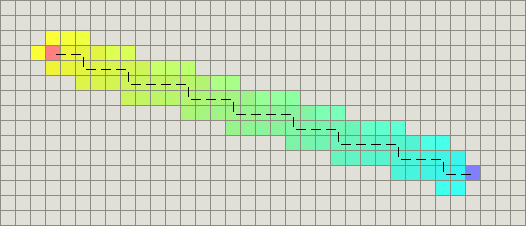
\includegraphics[scale=0.7]{manhattan.png}}
\caption{Манхэттенское расстояние}
\label{manh}
\end{figure}

\begin{figure}[h]
\center{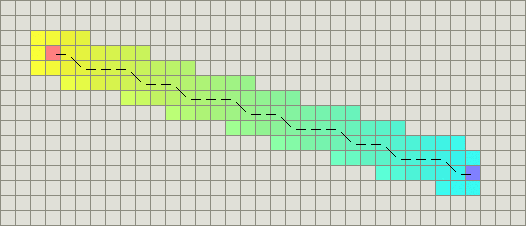
\includegraphics[scale=0.7]{diagonal.png}}
\caption{Диагональное расстояние}
\label{diag}
\end{figure}

\subsection{Реализация интерфейса}
\subsubsection{Внешная спецификация}
\subsubsection{Внутренняя спецификация}
\subsubsection{Пример работы}
\pagebreak
\section{Заключение}
В работе были рассмотрены два распространённых алгоритма поиска кратчайшего пути: A* и алгоритм Дейкстры.

В данной реализации использовался простой граф с одинаковой стоимостью рёбер. На практике же чаще всего идеальных условий не бывает. В сети дорог существуют разные типы дорог, поэтому необходимо установить разный вес рёбер: например, для асфальтированных дорог меньше, для просёлочных больше. Можно динамически редактировать вес, например, чтобы учитывать пробки: чем больше пробка, тем больше вес. Главное, соблюдать одинаковую размерность весов.

Чаще всего требуется быстрая работа алгоритма в условиях огромных карт. В реализованной программе для хранения данных используется список, что замедляет работу алгоритма, так как каждый раз приходится искать вершину с наименьшим коэффициентом и удалять её сдвигом. Для увеличения скорости можно использовать, например, бинарную кучу, тогда необходимо просто будет извлекать первый элемент.

На практике поиск кратчайшего пути за оптимальное время очень важен не только в устройствах навигации, но и в коммуникационной сфере и даже в искусственом интеллекте.
\pagebreak
\begin{thebibliography}{99}
\addcontentsline{toc}{section}{Список литературы}
\bibitem{Corman}
Кормен, Т., Лейзерсон, Ч., Ривест, Р. Алгоритмы: построение и анализ = Introduction to Algorithms. — 1-е. — М.: МЦНМО, 2000. — 960 с. — ISBN 5-900916-37-5.
\end{thebibliography}


\end{document}
